\documentclass[a4paper,oneside,12pt]{ctexart}
\usepackage{enumerate,geometry,graphicx,bm,mathrsfs,xcolor,varwidth,framed,amsfonts,amssymb,indentfirst,fancyhdr,listings,float}
\usepackage[colorlinks,linkcolor=red,anchorcolor=blue,citecolor=blue,urlcolor=blue]{hyperref}
\usepackage[thmmarks,hyperref]{ntheorem}
\usepackage{amsmath}
\usepackage{cleveref}

\setlength{\headheight}{15pt}
\newfontfamily\consolas{Consolas}
\allowdisplaybreaks[4]
\linespread{1.5}
\geometry{centering,left=2.54cm,right=2.54cm,top=3.18cm,bottom=3.18cm}
\pagestyle{fancy}
\fancyhead[L]{\kaishu 强基数学001}
\fancyhead[C]{\kaishu 张卓立}
\fancyhead[R]{\kaishu 2204110786}
\definecolor{matlabgreen}{rgb}{0,0.5,0}
\definecolor{matlabpurple}{rgb}{0.75,0,0.75}
\lstset{
    language=MATLAB,
    basicstyle=\consolas,
    keywordstyle=\color{blue},
    commentstyle=\color{matlabgreen}\itshape,
    stringstyle=\color{matlabpurple}\ttfamily,
    frame=single,
    numbers=left,
    numberstyle=\tiny\consolas,
    emph={mean,var,moment,unifit,unifrnd,ones,tpdf,normpdf},
    emphstyle=\color{blue}
}

{
    \theoremstyle{plain}
    \theoremheaderfont{\normalfont\bfseries}
    \theorembodyfont{\kaishu}
    \theoremseparator{.}
    \newtheorem{exercise}{习题}
}

{
    \theoremstyle{nonumberplain}
    \theoremheaderfont{\bfseries}
    \theorembodyfont{\normalfont}
    \newtheorem{solution}{结果.}
}

\crefname{exercise}{习题}{习题}
\crefname{figure}{图}{图}
\crefname{table}{表}{表}
\crefname{equation}{式}{式}

\newcommand{\dif}{\mathrm{d}}
\newcommand{\differ}{\backslash}
\newcommand{\ptl}{\partial}
\newcommand{\R}{\mathbb{R}}
\newcommand{\N}{\mathbb{N}}
\newcommand{\C}{\mathbb{C}}
\newcommand{\Z}{\mathbb{Z}}
\renewcommand{\phi}{\varphi}
\renewcommand{\epsilon}{\varepsilon}
\newcommand{\abs}[1]{\left\vert#1\right\vert}
\newcommand{\norm}[1]{\left\Vert#1\right\Vert}
\newcommand{\expect}{\mathbb{E}}
\newcommand{\var}{\mathrm{Var}}
\newcommand{\prob}{\mathbb{P}}
\newcommand{\Exp}{\mathrm{Exp}}
\newcommand{\poi}{\mathrm{Poi}}
\newcommand{\Beta}{\mathrm{Beta}}

\begin{document}
    \begin{center}
        \bfseries\LARGE
        数理统计编程作业
    \end{center}

    \begin{exercise}
        \label{ex:1}
        假设$X_1,\cdots,X_n$是来自总体$X$的随机样本,$X\sim\chi^2(k)$.

        (1) 求样本均值$\bar{X}$的密度函数.

        (2) 求样本均值的渐进分布.

        (3) 通过编程比较,在不同样本量下,样本均值的密度函数和其渐进分布的密度函数图像.
    \end{exercise}

    \begin{solution}
        代码如下:
        \begin{lstlisting}
%第一题
clear;clc;
k=6;n=5;
x=0:.1:15;
y=(1/2)^(n*k/2)/gamma(n*k/2)*(n.*x).^(n*k/2-1).*exp(-n*x/2)*n;
plot(x,y);
hold on;
yasym=normpdf(x,k,sqrt(2*k/n));
plot(x,yasym);
legend('样本均值n=5','渐进分布');
        \end{lstlisting}

        图像如图:
        \begin{figure}[H]
            \centering
            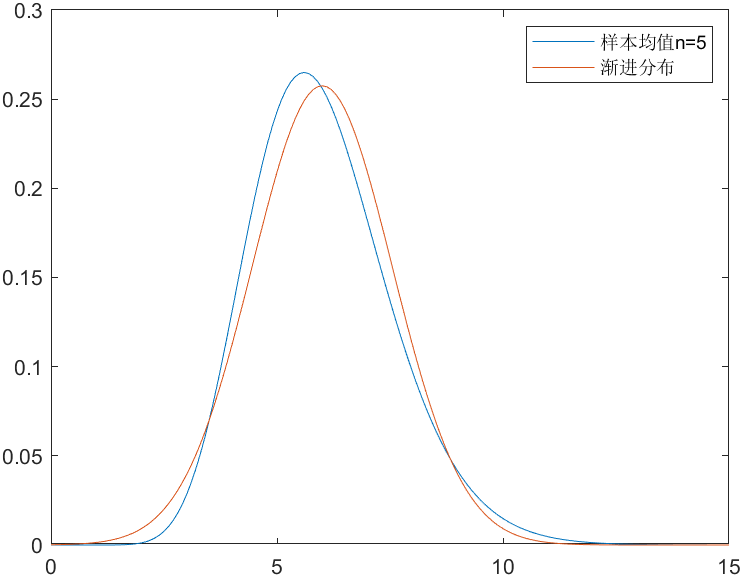
\includegraphics[scale=0.7]{第一问.png}
            \caption{第一题图}
        \end{figure}
    \end{solution}

    \begin{exercise}
        \label{ex:2}
        在一个图上画出标准正态分布的密度曲线和$t(1),t(3),t(30),t(100)$的密度曲线.
    \end{exercise}

    \begin{solution}
        代码:
        \begin{lstlisting}
%第二题
clear;clc;
x=-10:.1:10;
y1=normpdf(x);%标准正态分布
y2=tpdf(x,1);%t(1)分布
y3=tpdf(x,3);%t(3)分布
y4=tpdf(x,30);%t(30)分布
y5=tpdf(x,100);%t(100)分布
plot(x,y1);
hold on;
plot(x,y2);
plot(x,y3);
plot(x,y4);
plot(x,y5);
legend('标准正态分布','t=1','t=3','t=30','t=100');
hold off;
        \end{lstlisting}
        图像:
        \begin{figure}[H]
            \centering
            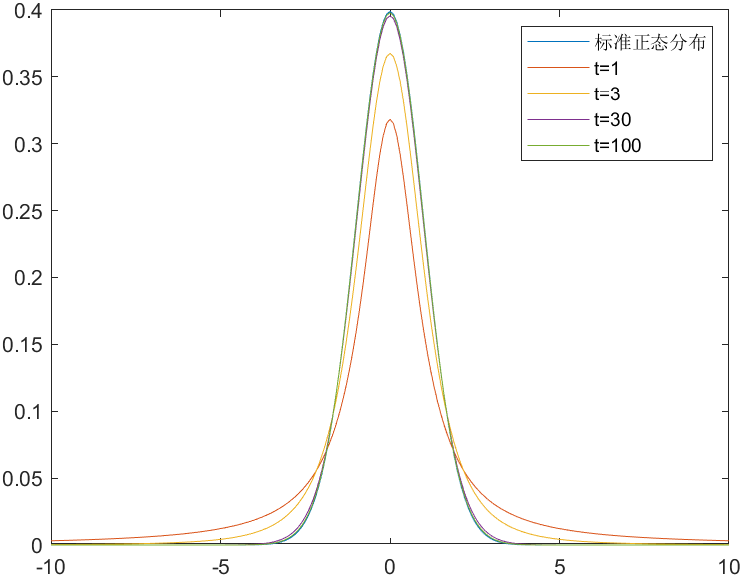
\includegraphics[scale=0.7]{第二问.png}
            \caption{第二题图}
        \end{figure}
    \end{solution}

    \begin{exercise}
        \label{ex:3}
        令$X_1,\cdots,X_n$是来自均匀分布$U[\mu-\sqrt{3}\sigma,\mu+\sqrt{3}\sigma]$的随机样本,其中$-\infty <\mu<\infty,\sigma>0$.编程比较$\mu$
        的矩估计和极大似然估计的偏,方差和均方误差.
    \end{exercise}

    \begin{solution}
        代码:
        \begin{lstlisting}
%第三题
clear;clc;
mu=0;sigma=2;
size=[1,1000];
a=mu-sqrt(sigma);b=mu+sqrt(sigma);
meanx=(a+b)/2;varx=(b-a)^2/12;
momentsampleset=zeros(1,100);
mlesampleset=zeros(1,100);
for k=1:100
    r=unifrnd(a,b,size);%选取随机样本
    momentsampleset(1,k)=mean(r);%样本矩估计
    mlesampleset(1,k)=unifit(r);%样本MLE
end
momentbias=meanx-mean(momentsampleset)%矩估计的偏
momentvar=var(momentsampleset)%矩估计的方差
momentmse=moment(momentsampleset-meanx*ones(1,100),2)
    %矩估计的MSE
mlebias=meanx-mean(mlesampleset)%极大似然估计的偏
mlevar=var(mlesampleset)%极大似然估计的方差
mlemse=moment(mlesampleset-meanx*ones(1,100),2)
    %极大似然估计的MSE
        \end{lstlisting}

        结果:
        \begin{lstlisting}

momentbias =

    0.0022


momentvar =

   7.3353e-04


momentmse =

   7.2620e-04


mlebias =

    1.4113


mlevar =

   9.1934e-06


mlemse =

   9.1015e-06

        \end{lstlisting}
    \end{solution}
\end{document}